	The equation of line in terms of vector notations can be written as
\begin{align}
	\vec{n}^T \vec{x} = c  
\end{align}
Let the intercepts be $\myvec{a \\ 0}$ and $\myvec{0 \\ b}$, respectively.

	Given that: \quad $ a + b = 1 $, \quad and \quad $ ab = -6$ 

The quadratic equation whose roots are the x and y intercepts can be written as:
\begin{align}
	x^2 - (\text{sum of roots})x &+ (\text{product of roots}) = 0 \\
	\implies \qquad & x^2 - x -6 =0 \\
	\implies \qquad & x=(3,-2) 
\end{align}
and corresponding $y$ intercepts are $(-2,3)$. 

The line $L_1$ passes through $\myvec{3 \\ 0}$ and $\myvec{0 \\ -2}$.

%.............................................................................
Let direction vector of this line be $\vec{m}$.
\begin{align}
	\vec{m} = \myvec{0\\-2} - \myvec{3\\0} = \myvec{-3\\-2}
\end{align}
The normal vector, $\vec{n}$: 
\begin{align}
	{\vec{n}} = \myvec{0 & -1 \\ 1 & 0}\vec{m} = \myvec{2 \\ -3}
\end{align}
%.............................................................................
The equation of line in terms of normal vector and passing through a point $A$ 
	is
\begin{align}
	\quad \vec{n^T}(\vec{x} - A ) = 0
	\quad \implies \quad \vec{n^Tx} = \vec{n^T}A \\
	\implies \vec{n^Tx}= \myvec{2 -3}\myvec{3 \\ 0} \\
	\implies \myvec{2 -3}\vec{x} = 6	\label{eq:solutions/line_plane_45/L1}
\end{align}
Similarly, the equation of second line $L_2$, with $x$ and 
	$y$ intercepts $\myvec{ -2 \\ 0}$ and $\myvec{ 0 \\ 3}$ and 
	normal vector $\myvec{ -3 \\ 2}$ is
\begin{align}
	\myvec{-3 &  2 } {\vec{x}} = 6	\label{eq:solutions/line_plane_45/L2}
\end{align}
The equations of lines (\ref{eq:solutions/line_plane_45/L1}) and (\ref{eq:solutions/line_plane_45/L2}) can be represented 
	collectively as
\begin{align}
	\myvec{2 & -3 \\ -3 & 2}\vec{x} = \myvec{6 \\ 6}
\end{align}

%.............................................................................
\begin{table}[htbp]
	\centering
	\begin{tabular}{|c|c|c|} \hline 
	$x-$intercept & $y-$intercept & \quad $\vec{n}$  \\ \hline \hline
	\myvec{3\\0}	&	\myvec{0\\-2}	&	\myvec{2\\-3} \\ \hline
	\myvec{-2\\0}	&	\myvec{0\\3}	&	\myvec{-3\\2} \\ \hline
	\end{tabular}
	\caption{} \label{coeftable}
\end{table}
%.............................................................................
\begin{figure}[!h]
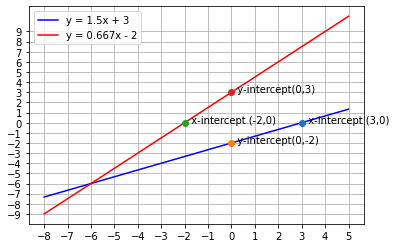
\includegraphics[width=\columnwidth]{./solutions/line_plane_45/stline_plot.png}
	\caption{}  \label{linefig1:solutions/line_plane_45/} 
\end{figure}

\end{document}
